\documentclass[11pt,a4paper]{article}

% ---------- encoding / fonts ----------
\usepackage[utf8]{inputenc}
\usepackage[T1]{fontenc}
\usepackage{textcomp}
\usepackage{mathpazo}           % Palatino body serif
\usepackage[scaled=0.92]{helvet} % Helvetica for sans headings
\renewcommand{\ttdefault}{cmtt}  % Computer Modern Typewriter for code

% ---------- layout ----------
\usepackage[a4paper,margin=2.6cm,headheight=14pt]{geometry}
\usepackage{fancyhdr}
\usepackage{titlesec}
\usepackage{enumitem}
\usepackage{multicol}
\usepackage{array}
\usepackage{booktabs}
\usepackage{longtable}
\usepackage{caption}
\usepackage{graphicx}
\usepackage{tikz}
\usetikzlibrary{arrows.meta,positioning,calc}
\usepackage[most]{tcolorbox}
\usepackage{fancyvrb}
\usepackage{xcolor}
\usepackage[hidelinks]{hyperref}
\usepackage{parskip}

\setlength{\parskip}{0.55\baselineskip}
\setlength{\parindent}{0pt}

% ---------- palette ----------
\definecolor{inkc}{HTML}{14171C}
\definecolor{inksoft}{HTML}{4A505E}
\definecolor{inkfaint}{HTML}{767D8C}
\definecolor{linec}{HTML}{C9CED7}
\definecolor{linestrong}{HTML}{A9B1BE}
\definecolor{accentc}{HTML}{B65A0C}
\definecolor{accentink}{HTML}{7A3F06}
\definecolor{accentsoft}{HTML}{F4E2C8}
\definecolor{redc}{HTML}{A13A2C}
\definecolor{redsoft}{HTML}{F4DDD7}
\definecolor{greenc}{HTML}{276B48}
\definecolor{greensoft}{HTML}{DBEEE2}
\definecolor{consolebg}{HTML}{14171D}
\definecolor{consoleink}{HTML}{D8DEE8}
\definecolor{tablehead}{HTML}{F3F4F7}

\color{inkc}

% ---------- section styling ----------
\titleformat{\section}
  {\normalfont\sffamily\bfseries\Large\color{inkc}}
  {\color{accentink}\thesection}{0.6em}{}
\titleformat{\subsection}
  {\normalfont\sffamily\bfseries\large\color{inkc}}
  {\color{accentink}\thesubsection}{0.6em}{}
\titlespacing*{\section}{0pt}{1.6em}{0.8em}
\titlespacing*{\subsection}{0pt}{1.2em}{0.5em}

% ---------- header/footer ----------
\pagestyle{fancy}
\fancyhf{}
\renewcommand{\headrulewidth}{0.4pt}
\renewcommand{\footrulewidth}{0pt}
\fancyhead[L]{\small\sffamily\color{inkfaint} Trust Me, I'm a Camera}
\fancyhead[R]{\small\sffamily\color{inkfaint} \nouppercase{\leftmark}}
\fancyfoot[C]{\small\sffamily\color{inkfaint} \thepage}

% ---------- hyperref ----------
\hypersetup{
  colorlinks=true,
  linkcolor=accentink,
  citecolor=accentink,
  urlcolor=accentink,
  pdftitle={Trust Me, I'm a Camera},
  pdfauthor={Mart{\'i}n L{\'o}pez Aranburu},
  pdfsubject={RTSP/RTP man-in-the-middle and frame-injection attack against video-surveillance systems},
  pdfkeywords={RTSP, RTP, RTCP, MITM, ARP spoofing, video surveillance, IoT security}
}

% ---------- callout boxes ----------
\newtcolorbox{notebox}[1][]{
  enhanced, breakable, colback=white, colframe=linec, boxrule=0.5pt,
  left=11pt, right=9pt, top=6pt, bottom=6pt,
  borderline west={2.6pt}{0pt}{accentc},
  before upper={\sffamily\bfseries\small\color{accentink}#1\par\vspace{2pt}\normalfont\rmfamily\normalsize\color{inkc}}
}
\newtcolorbox{cautionbox}[1][]{
  enhanced, breakable, colback=white, colframe=linec, boxrule=0.5pt,
  left=11pt, right=9pt, top=6pt, bottom=6pt,
  borderline west={2.6pt}{0pt}{redc},
  before upper={\sffamily\bfseries\small\color{redc}#1\par\vspace{2pt}\normalfont\rmfamily\normalsize\color{inkc}}
}
\newtcolorbox{fieldbox}[1][]{
  enhanced, breakable, colback=white, colframe=linec, boxrule=0.5pt,
  left=11pt, right=9pt, top=6pt, bottom=6pt,
  borderline west={2.6pt}{0pt}{greenc},
  before upper={\sffamily\bfseries\small\color{greenc}#1\par\vspace{2pt}\normalfont\rmfamily\normalsize\color{inkc}}
}
\newtcolorbox{consolebox}{
  enhanced, breakable, colback=consolebg, colframe=consolebg,
  left=10pt, right=10pt, top=7pt, bottom=7pt, boxrule=0pt, sharp corners, arc=2pt,
  fontupper=\ttfamily\small\color{consoleink}
}
\DefineVerbatimEnvironment{consolev}{Verbatim}{fontsize=\small,commandchars=\\\{\}}

% ---------- figure caption style ----------
\captionsetup{font={sf,small,color=inkfaint},labelfont={bf,color=accentink},skip=6pt}

% ---------- small helpers ----------
\newcommand{\code}[1]{\texttt{\small #1}}
\newcommand{\paperto}{$\rightarrow$}
\newcommand{\paperlr}{$\leftrightarrow$}

\begin{document}
\thispagestyle{empty}

% =====================================================================
% MASTHEAD
% =====================================================================
\begin{center}
{\sffamily\footnotesize
 \colorbox{tablehead}{\strut\textcolor{inksoft}{\;TECHNICAL PAPER\;}}\hspace{4pt}%
 \colorbox{accentsoft}{\strut\textcolor{accentink}{\;\bfseries EDUCATIONAL \& AUTHORIZED-TESTING USE ONLY\;}}\hspace{4pt}%
 \colorbox{tablehead}{\strut\textcolor{inksoft}{\;V1 \textperiodcentered\ SEPTEMBER 2026\;}}
}
\end{center}
\vspace{14pt}

{\centering\sffamily\bfseries\fontsize{28}{32}\selectfont Trust Me, I'm a Camera\par}
\vspace{6pt}
{\centering\itshape\large\color{inksoft} A man-in-the-middle and RTP replay attack against RTSP video-surveillance streams\par}
\vspace{12pt}
{\centering\sffamily\small
Mart\'in L\'opez Aranburu \quad\textbullet\quad linkedin.com/in/mart\'in-l\'opez-aranburu \quad\textbullet\quad Barcelona Cybersecurity Congress, November 2026
\par}
\vspace{18pt}

\begin{tcolorbox}[enhanced, colback=white, colframe=linec, boxrule=0.6pt, left=16pt,right=16pt,top=10pt,bottom=10pt]
{\sffamily\bfseries\footnotesize\color{accentink} ABSTRACT}\par\vspace{4pt}
RTSPoofing is a working man-in-the-middle tool that defeats the RTSP/RTP pipeline used by the large majority of consumer and small-business IP cameras and network video recorders (NVRs). By combining ARP-based network positioning with a byte-transparent RTSP relay and RTP-level frame substitution, an on-path attacker can silently replace a live camera feed with pre-recorded footage while the recording NVR continues to log a fully valid-looking stream --- correct sequence numbers, correct timestamps, correct sender identity, and, optionally, a forged RTCP wall-clock. This paper documents the attack's three-stage architecture, its extension to UDP-transported RTP, a field observation about switch MAC-address-table learning that let the attack proceed on a network configured with Dynamic ARP Inspection, and the concrete defenses that close each stage.
\par\vspace{8pt}
{\sffamily\bfseries\footnotesize\color{inkfaint} KEYWORDS\;\;}{\footnotesize\color{inksoft}RTSP \textperiodcentered\ RTP/RTCP \textperiodcentered\ man-in-the-middle \textperiodcentered\ ARP spoofing \textperiodcentered\ video surveillance \textperiodcentered\ IoT/embedded security \textperiodcentered\ protocol authentication}
\end{tcolorbox}

\vspace{6pt}
{\small\tableofcontents}

\newpage

% =====================================================================
\section{Introduction}
\emph{Physical security infrastructure runs on network infrastructure, and the network infrastructure it runs on was never designed to authenticate itself.}

The large majority of IP cameras and the NVRs that record them speak RTSP in plaintext, negotiate an RTP media session with no cryptographic integrity, and trust whatever arrives on the negotiated channel. This paper asks a narrow, concrete question: what does it actually take to make an NVR record a fabricated feed --- without touching camera or NVR firmware, without credentials, and without the NVR ever registering an anomaly --- and where, specifically, does that stop working?

The answer is implemented as \textbf{RTSPoofing}, an asynchronous Rust/Tokio proxy (\raise0.3ex\hbox{$\scriptstyle\sim$}1{,}600 lines across eight modules) that performs the attack end-to-end against both transport modes RTSP supports. Sections~4--7 walk through its three-stage pipeline and its UDP extension in the order the implementation executes them. Section~8 documents an unplanned field finding --- a switch's own MAC-learning behavior undermining a correctly configured Dynamic ARP Inspection policy on a segmented corporate network. Sections~9--11 scope what was and wasn't verified, and Section~10 maps each stage to a specific, low-cost defense.

\begin{notebox}[SCOPE]
All testing described here was performed in isolated lab environments or under explicit written authorization. Findings labeled \emph{informal} or \emph{field observation} come from the author's own test environments and are not a controlled study across a representative device population --- see \S9 and \S11 for the specific caveats.
\end{notebox}

% =====================================================================
\section{Background: RTSP and RTP}
RTSP (Real Time Streaming Protocol, RFC~2326) is the out-of-band control channel almost every IP camera speaks: a client --- here, the NVR --- issues text requests to negotiate and control a media session.

\begin{consolebox}
\begin{consolev}
\textcolor{consoleink!60}{NVR -> CAM}  DESCRIBE rtsp://192.168.1.64/stream RTSP/1.0
\textcolor{consoleink!60}{CAM -> NVR}  200 OK -- SDP body: available media, codecs, transport options

\textcolor{consoleink!60}{NVR -> CAM}  SETUP rtsp://192.168.1.64/stream/track1 RTSP/1.0
              Transport: RTP/AVP;unicast;client_port=8000-8001
\textcolor{consoleink!60}{CAM -> NVR}  200 OK -- Transport: ...;server_port=9000-9001  \textcolor{accentc}{(or interleaved=0-1)}

\textcolor{consoleink!60}{NVR -> CAM}  PLAY rtsp://192.168.1.64/stream RTSP/1.0
\textcolor{consoleink!60}{CAM -> NVR}  200 OK -- media now flowing
\end{consolev}
\end{consolebox}

The \code{SETUP} exchange is the detail this paper returns to repeatedly: it negotiates one of two transports for the RTP/RTCP that follows. \textbf{TCP-interleaved} frames the media inside the same RTSP connection, each frame prefixed with a \code{\$} marker, a channel number, and a 2-byte length (RFC~2326 \S10.4). \textbf{UDP} instead sends RTP and RTCP as independent datagrams on the \code{client\_port}/\code{server\_port} pairs exchanged during \code{SETUP}. Both are common in the field; \S7 covers why the UDP case needs separate handling.

\subsection{The RTP header}
Once negotiated, media flows as a sequence of RTP packets (RFC~3550). Three header fields carry the entire state a receiver uses to make sense of the stream:

\begin{consolebox}
\begin{consolev}
 0                   1                   2                   3
 0 1 2 3 4 5 6 7 8 9 0 1 2 3 4 5 6 7 8 9 0 1 2 3 4 5 6 7 8 9 0 1
+-+-+-+-+-+-+-+-+-+-+-+-+-+-+-+-+-+-+-+-+-+-+-+-+-+-+-+-+-+-+-+-+
|V=2|P|X|  CC   |M|     PT      |       Sequence Number        |
+-+-+-+-+-+-+-+-+-+-+-+-+-+-+-+-+-+-+-+-+-+-+-+-+-+-+-+-+-+-+-+-+
|                           Timestamp                           |
+-+-+-+-+-+-+-+-+-+-+-+-+-+-+-+-+-+-+-+-+-+-+-+-+-+-+-+-+-+-+-+-+
|           Synchronization Source (SSRC) identifier            |
+-+-+-+-+-+-+-+-+-+-+-+-+-+-+-+-+-+-+-+-+-+-+-+-+-+-+-+-+-+-+-+-+
\end{consolev}
\end{consolebox}

\begin{center}
\small
\begin{tabular}{@{}p{4.1cm}p{10.6cm}@{}}
\toprule
\textbf{\textcolor{accentink}{Sequence Number}} & 16-bit, increments per packet. RTP runs over lossy UDP by design, so conforming receivers conceal isolated gaps rather than terminating the session (RFC~3550 \S8). A large or backward discontinuity is what actually surfaces as a defect. \\[4pt]
\textbf{\textcolor{accentink}{Timestamp}} & 32-bit media clock, conventionally 90~kHz for video regardless of frame rate. Should advance monotonically; a stall or reversal is what a jitter buffer notices. \\[4pt]
\textbf{\textcolor{accentink}{SSRC}} & 32-bit sender identity. A receiver is expected to treat a change as a new source and reset decoder state (RFC~3550 \S8.2) --- disruptive to conceal, not fatal to avoid. \\
\bottomrule
\end{tabular}
\end{center}

None of these fields carry a signature or MAC. SRTP (RFC~3711) adds exactly that and is, practically, absent from consumer and SMB CCTV. Three unauthenticated fields are the entire surface the rest of this paper manipulates.

% =====================================================================
\section{Threat model and architecture}
The attacker is assumed to share a broadcast domain (an unsegmented VLAN) with the camera and the NVR --- the common case among the deployments surveyed in \S9 --- and to hold no camera or NVR credentials. The goal is not to exfiltrate the stream but to substitute its \emph{content} while the NVR continues to believe it is recording the camera live.

\begin{figure}[h]
\centering
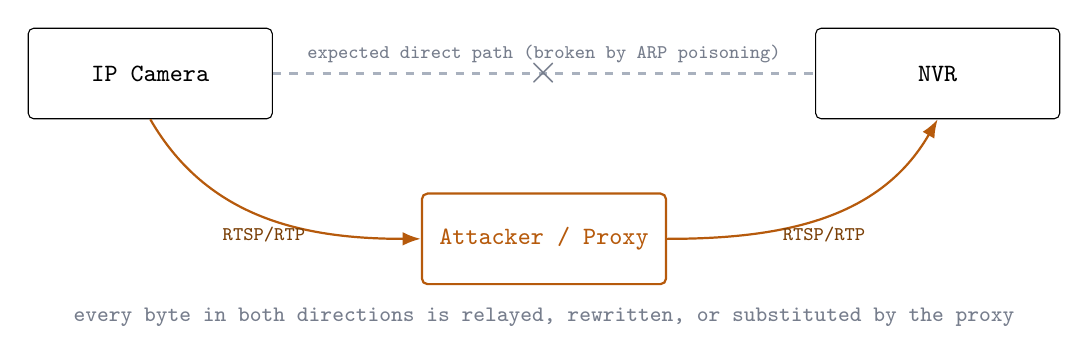
\begin{tikzpicture}[
  box/.style={draw, rounded corners=2pt, minimum width=3.1cm, minimum height=1.15cm, font=\ttfamily\small, align=center},
  abox/.style={box, draw=accentc, thick, text=accentc, font=\ttfamily\small\bfseries},
  lbl/.style={font=\ttfamily\scriptsize, text=inksoft},
  >=Latex
]
\node[box] (cam) at (0,0) {IP Camera};
\node[box] (nvr) at (10,0) {NVR};
\node[abox] (atk) at (5,-2.1) {Attacker / Proxy};

\draw[dashed, linestrong, thick] (cam.east) -- (nvr.west)
  node[midway, above, lbl, text=inkfaint]{expected direct path (broken by ARP poisoning)};
\node at (5,0) {\Large\color{inkfaint}$\times$};

\draw[->, accentc, thick] (cam.south) to[out=-60,in=180] node[midway,below,lbl,text=accentink]{RTSP/RTP} (atk.west);
\draw[->, accentc, thick] (atk.east) to[out=0,in=-120] node[midway,below,lbl,text=accentink]{RTSP/RTP} (nvr.south);

\node[lbl, text=inkfaint] at (5,-3.1) {\footnotesize every byte in both directions is relayed, rewritten, or substituted by the proxy};
\end{tikzpicture}
\caption{ARP spoofing does not open a new path --- it breaks the one the camera and NVR believe they're using, and both sides' traffic is redirected through the attacker instead.}
\end{figure}

The implementation executes this as three stages, one \code{MITMSession} task per accepted TCP connection:
\begin{enumerate}[leftmargin=1.4em, itemsep=2pt]
\item \textbf{Phase I --- network-layer positioning} (\S4): ARP spoofing places the attacker on-path at layer~2.
\item \textbf{Phase II --- transparent interception} (\S5): a byte-level RTSP/RTP relay with live parameter auto-detection.
\item \textbf{Phase III --- media substitution} (\S6): paced, continuity-preserving RTP frame injection.
\end{enumerate}

Both supported transports (TCP-interleaved and UDP, \S7) are routed through the same frame-handling function, \code{process\_camera\_frame()}, specifically so probing, capture, and injection behavior cannot silently diverge between them.

% =====================================================================
\section{Phase I --- network-layer positioning}
Camera and NVR normally address each other directly. The attacker poisons both ARP caches with periodic forged replies --- conventionally via a tool such as \code{arpspoof} --- so each side resolves the other's IP to the attacker's MAC address:

\begin{consolebox}
\begin{consolev}
arpspoof -i eth0 -t <NVR> <CAM>
arpspoof -i eth0 -t <CAM> <NVR>
\end{consolev}
\end{consolebox}

With IP forwarding enabled on the attacker host, traffic continues to flow end-to-end and neither side's link appears to break --- it now simply routes through the attacker first. This is a standard, well-documented technique; its only requirement is layer-2 adjacency, which is the normal case for camera and NVR on a flat, unsegmented network (\S9).

\begin{cautionbox}[WHAT STOPS IT]
Dynamic ARP Inspection (DAI) validates ARP packets against a DHCP-snooping or static binding table and drops ones that don't match, which is a complete stop for this phase in isolation. \S8 documents a case where DAI was correctly configured and this phase still succeeded --- not because DAI failed, but because of an unrelated switch behavior.
\end{cautionbox}

% =====================================================================
\section{Phase II --- transparent interception}
With traffic flowing through it, the proxy does two things concurrently: relay the RTSP control channel byte-for-byte, and passively characterize the RTP media it's relaying.

\subsection{Byte-transparent RTSP relay, credentials included}
An \code{RtspTextScanner} accumulates raw TCP bytes and emits complete RTSP messages as they become available --- boundaries are the header block's terminating blank line plus any \code{Content-Length} body, exactly mirroring how a stateful \code{InterleavedParser} on the media side finds complete \code{\$}-framed RTP frames. Every RTSP request and response is forwarded unmodified \emph{except} where a UDP \code{SETUP} exchange requires a Transport-header rewrite (\S7).

This includes any \code{Authorization} header. RTSP supports Basic and Digest authentication on these same requests, and a meaningful share of real deployments enable it --- but the proxy never needs to know the camera's password. The NVR computes its own credentials exactly as it always does and sends them through a connection it believes is direct; the proxy simply relays that header like every other byte. Camera authentication protects against a new, unauthorized client opening a session. It does not protect a session between two already-authorized parties from an on-path relay that was never asked to authenticate at all.

\subsection{RTPProbe: live parameter detection}
Rather than requiring the operator to specify payload type, SSRC, or frame rate up front, the proxy derives them from the live stream during a short warm-up window. Each RTP frame updates a majority vote over payload type, SSRC, and (for the interleaved case) channel number; the value with the most occurrences by the time the window closes (a configurable duration \emph{and} a minimum frame count) is taken as ground truth --- deliberately not just the first packet seen, since the packets immediately after \code{PLAY} are often noisy.

\begin{consolebox}
\begin{consolev}
\textcolor{consoleink!60}{[00:00.0]} Analyzing stream...
\textcolor{consoleink!60}{[00:01.2]} PT=96 seen 847 times -> dynamic H264
\textcolor{consoleink!60}{[00:02.1]} SSRC=0xDEAD1234 dominant (99.8% of frames)
\textcolor{consoleink!60}{[00:02.8]} Estimated FPS: 25.0 Hz (via RTP timestamp deltas)
\textcolor{consoleink!60}{[00:03.0]} Codec: H264 (fragmented FU-A detected)
\textcolor{greenc}{[00:03.0]} Probe complete -- starting injection
\end{consolev}
\end{consolebox}

Frame rate specifically is derived without any out-of-band signaling, using only the fact that RTP's video clock runs at a fixed, standard 90{,}000~Hz regardless of the actual frame rate: sampling consecutive packets' RTP timestamp deltas and taking the \emph{median} across a sliding window (up to the last 60 valid samples, filtering deltas that wrap, exceed one clock period, or arrive with an implausibly small wall-clock gap) converges on

\begin{consolebox}
\begin{consolev}
fps = 90000 / dts

e.g.  3,600 ticks between two frames -> 90000 / 3600 = \textcolor{accentc}{25 fps}
\end{consolev}
\end{consolebox}

% =====================================================================
\section{Phase III --- media substitution}
Once parameters are known, an injector replaces the live stream with frames read from a \code{.rtp} capture file --- either recorded earlier from the same camera in the proxy's own \code{record} mode (an 8-byte record header plus raw RTP payload per frame, written on a dedicated blocking task so a slow disk never stalls the live relay, see Appendix~A), or synthesized from any source video with \code{ffmpeg}.

\subsection{Continuity rewrite}
Every injected frame's sequence number and timestamp are rewritten to continue, monotonically, from the last values observed on the \emph{live} stream at the moment injection starts, and the SSRC is set to the one the real camera was using (or an explicit operator override). The transition from live to injected is therefore invisible at the RTP-metadata level: there is no gap, no reversal, and no change of apparent source for a receiver to key off.

\subsection{Fixed-rate pacing}
Frames are emitted on a \code{tokio::time::interval} ticking once per \code{1/fps} seconds, configured with \code{MissedTickBehavior::Delay}: a slow write or scheduler hiccup delays the next tick rather than bursting subsequent frames to catch up. An unpaced injector that simply emits frames as fast as the network allows is, in practice, the easiest way for this kind of attack to get noticed --- dropped or corrupted frames and visibly bursty inter-arrival timing are exactly the sort of signal that stands out even to something that never decodes a single frame.

\subsection{Two independent notions of ``now''}
Cameras commonly carry two separate timestamps: an on-screen OSD burned into the pixels by camera firmware, and an RTCP Sender Report's NTP field --- a wall-clock value some VMS or forensic export tooling reads independently of the picture. Spoofing the first is free: an injected clip carries whatever OSD timestamp it was recorded with. The proxy additionally fabricates its own SR every \code{rtcp\_sr\_interval} seconds, stamped with the real current time, tracking the injected stream's own packet and octet counts:

\begin{center}
\small
\begin{tabular}{@{}lll@{}}
\toprule
\textbf{Bytes} & \textbf{Field} & \textbf{Content} \\
\midrule
0--4   & \code{Header}         & V=2, P=0, RC=0 \textperiodcentered\ PT=200 (SR) \textperiodcentered\ length=6 words \\
4--8   & \code{SSRC}           & Sender identifier --- matches the injected stream's SSRC \\
8--12  & \code{NTP seconds}    & Wall-clock ``now'' at send time \\
12--16 & \code{NTP fraction}   & Sub-second wall-clock precision \\
16--20 & \code{RTP timestamp}  & Media-clock value at this instant, same clock as the stream \\
20--24 & \code{Packet count}   & Running total for this synthetic sender \\
24--28 & \code{Octet count}    & Running payload byte total \\
\bottomrule
\end{tabular}
\end{center}

The more consequential finding here is not the RTCP mechanics but the ordering of what matters: spoofing the picture already defeats the audience that matters most --- a human reviewing footage. RTCP timestamp forgery only matters against tooling that reads the wall clock instead of the frame; it is included for completeness against that narrower, more technical audience, not because it is the headline exposure.

% =====================================================================
\section{Extending to UDP transport}
Everything in \S5--\S6 was described for TCP-interleaved media. RTSP's \code{SETUP} just as commonly negotiates plain UDP --- independent RTP/RTCP datagrams on their own ports --- and that case needs different handling for a reason that's easy to gloss over: ARP spoofing places the attacker on-path at \emph{layer 2}, but with standard IP forwarding enabled, a UDP datagram addressed to the NVR's or camera's real IP is routed transparently by the kernel at the IP layer without ever reaching the proxy's own sockets. Being on-path at L2 is not the same as being on-path at the application layer; injecting into UDP media requires actually owning the datagrams, which means acting at the layer where the transport itself is negotiated --- the \code{SETUP} exchange.

The fix rewrites that negotiation the same way ARP spoofing rewrites the network below it, one layer up:
\begin{enumerate}[leftmargin=1.4em, itemsep=2pt]
\item The NVR's \code{SETUP} declares \code{client\_port=8000-8001}; the proxy substitutes ports it owns before forwarding the request to the camera.
\item The camera, none the wiser, now sends its RTP/RTCP straight to the proxy.
\item The camera's response declares \code{server\_port=9000-9001}; the proxy substitutes ports it owns there too, and restores the NVR's own original \code{client\_port} in the same response so the NVR isn't confused by a value it never sent.
\item The NVR, none the wiser, now sends its RTCP receiver reports straight to the proxy as well.
\end{enumerate}

\begin{figure}[h]
\centering
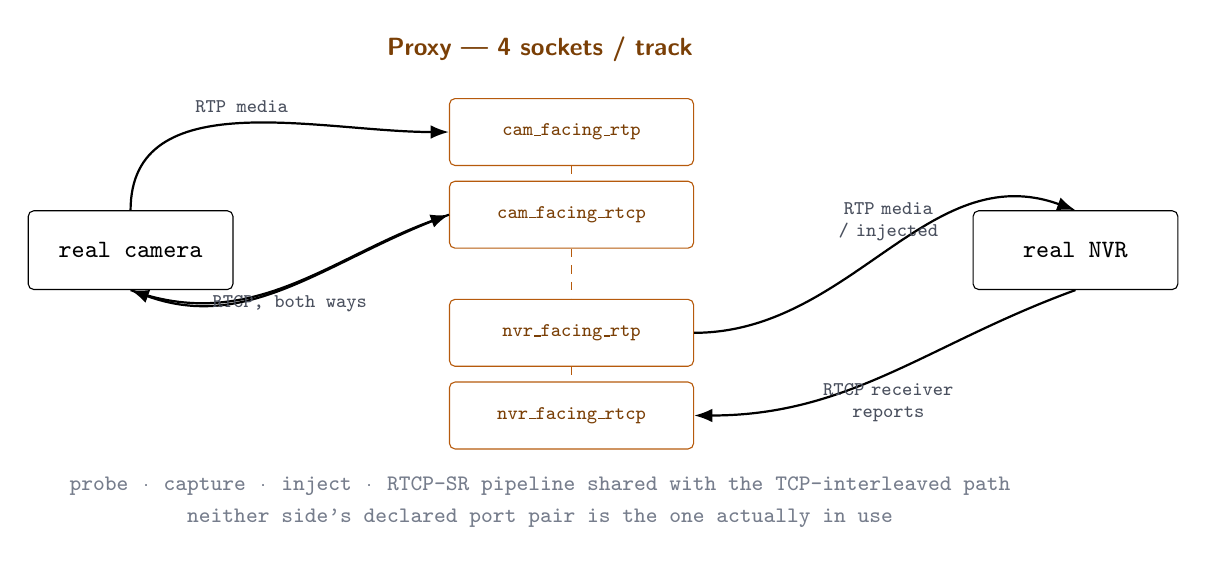
\begin{tikzpicture}[
  ebox/.style={draw, rounded corners=2pt, minimum width=2.6cm, minimum height=1cm, font=\ttfamily\small, align=center},
  sbox/.style={draw=accentc, rounded corners=2pt, minimum width=3.1cm, minimum height=0.85cm, font=\ttfamily\scriptsize, align=center, text=accentink},
  lbl/.style={font=\ttfamily\scriptsize, text=inksoft},
  >=Latex
]
\node[ebox] (cam) at (0,-1.5) {real camera};
\node[ebox] (nvr) at (12.0,-1.5) {real NVR};

\node[sbox] (crtp)  at (5.6, 0)    {cam\_facing\_rtp};
\node[sbox] (crtcp) at (5.6,-1.05) {cam\_facing\_rtcp};
\node[sbox] (nrtp)  at (5.6,-2.55) {nvr\_facing\_rtp};
\node[sbox] (nrtcp) at (5.6,-3.6)  {nvr\_facing\_rtcp};

\draw[->, thick] (cam.north) to[out=90,in=180] node[midway,above,lbl]{RTP media} (crtp.west);
\draw[->, thick] (crtcp.west) to[out=200,in=-20] (cam.south);
\draw[->, thick] (cam.south) to[out=-20,in=200] node[midway,below,lbl]{RTCP, both ways} (crtcp.west);

\draw[->, thick] (nrtp.east) to[out=0,in=160] node[midway,above,lbl,text width=3cm,align=center]{RTP media\\/ injected} (nvr.north);
\draw[->, thick] (nvr.south) to[out=200,in=0] node[midway,below,lbl,text width=3cm,align=center]{RTCP receiver\\reports} (nrtcp.east);

\draw[accentc, dashed] (crtp.south) -- (crtcp.north);
\draw[accentc, dashed] (crtcp.south) -- (nrtp.north);
\draw[accentc, dashed] (nrtp.south) -- (nrtcp.north);

\node[font=\sffamily\bfseries\small, text=accentink] at (5.2,1.05) {Proxy --- 4 sockets / track};
\node[lbl, text=inkfaint] at (5.2,-4.5) {\footnotesize probe \textperiodcentered\ capture \textperiodcentered\ inject \textperiodcentered\ RTCP-SR pipeline shared with the TCP-interleaved path};
\node[lbl, text=inkfaint] at (5.2,-4.9) {\footnotesize neither side's declared port pair is the one actually in use};
\end{tikzpicture}
\caption{Four sockets, not two: each side's real port pair is rewritten to one the proxy owns, so both media \emph{and} RTCP reports terminate at the proxy in both directions.}
\end{figure}

The rationale for four sockets rather than two: some NVR/camera implementations validate that received RTP/RTCP actually originates from the exact port pair declared during \code{SETUP}, so relaying or injecting media has to send from the socket each side was told about, not merely any socket that happens to reach them. This is a defensive design choice carried in the implementation --- it was not verified against a specific catalog of NVR/camera firmware, a limitation restated explicitly in \S11.

All four sockets feed the same \code{process\_camera\_frame()} path used for TCP-interleaved media, so probing, capture, injection, and RTCP forgery cannot silently diverge between the two transports --- auto-detection, pacing, and forged timestamps behave identically regardless of which one a given camera happens to use.

% =====================================================================
\section{Field observation: MAC-address-table learning}
One test network was a segmented, managed corporate environment with, as far as could be determined, Dynamic ARP Inspection enabled --- the expectation going in was that forged ARP replies would simply be dropped and Phase~I would go no further.

\begin{fieldbox}[OBSERVED (HIGH CONFIDENCE)]
After ARP spoofing began, a packet capture on the attacker host showed the switch's forwarding table relearn the camera's MAC address onto the attacker's switch port. The pre-existing camera\paperlr{}NVR TCP session subsequently reset, and the NVR's own reconnect logic established a new session --- this time through the proxy.
\end{fieldbox}

\begin{figure}[h]
\centering
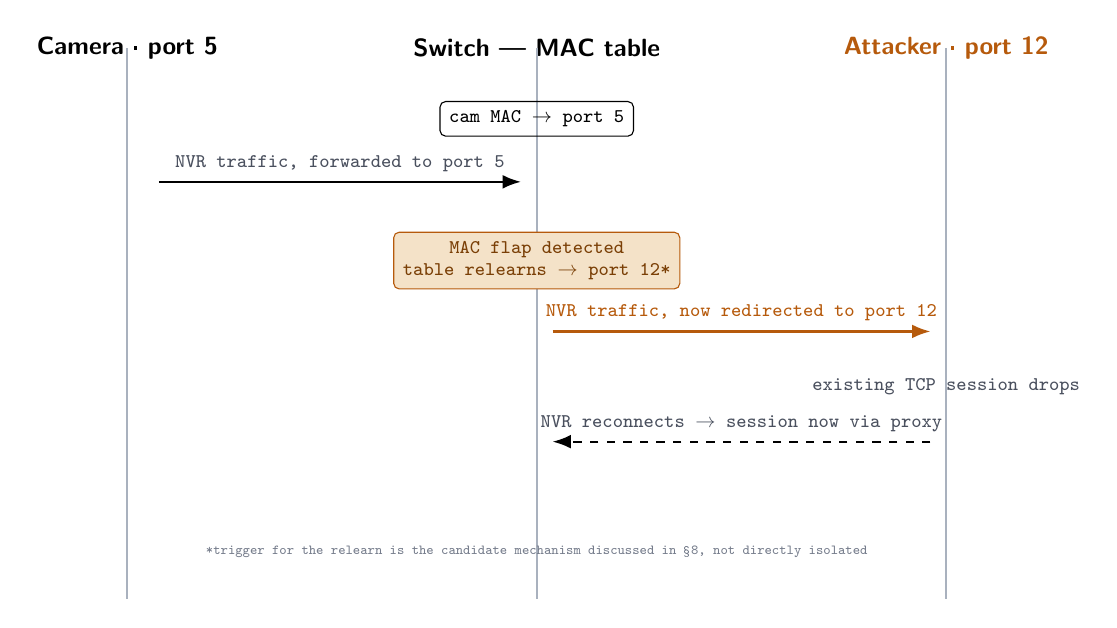
\begin{tikzpicture}[
  lifeline/.style={draw=linestrong, thick},
  evbox/.style={draw=accentc, fill=accentsoft, rounded corners=2pt, font=\ttfamily\scriptsize, align=center, text=accentink},
  lbl/.style={font=\ttfamily\scriptsize, text=inksoft},
  >=Latex
]
\node[font=\sffamily\bfseries\small] (l1) at (0,0)   {Camera \textperiodcentered\ port 5};
\node[font=\sffamily\bfseries\small] (l2) at (5.2,0) {Switch --- MAC table};
\node[font=\sffamily\bfseries\small, text=accentc] (l3) at (10.4,0) {Attacker \textperiodcentered\ port 12};

\draw[lifeline] (0,0) -- (0,-7);
\draw[lifeline] (5.2,0) -- (5.2,-7);
\draw[lifeline] (10.4,0) -- (10.4,-7);

\node[draw, rounded corners=2pt, font=\ttfamily\scriptsize] (t0) at (5.2,-0.9) {cam MAC \paperto\ port 5};

\draw[->,thick] (0.4,-1.7) -- (5.0,-1.7) node[midway, above, lbl]{NVR traffic, forwarded to port 5};

\node[evbox] (flap) at (5.2,-2.7) {MAC flap detected\\ table relearns \paperto\ port 12*};

\draw[->,accentc,thick] (5.4,-3.6) -- (10.2,-3.6) node[midway, above, lbl, text=accentc]{NVR traffic, now redirected to port 12};

\node[lbl] at (10.4,-4.3) {existing TCP session drops};

\draw[->,thick,dashed] (10.2,-5.0) -- (5.4,-5.0) node[midway, above, lbl]{NVR reconnects \paperto\ session now via proxy};

\node[lbl, text=inkfaint, font=\ttfamily\tiny] at (5.2,-6.4) {*trigger for the relearn is the candidate mechanism discussed in \S8, not directly isolated};
\end{tikzpicture}
\caption{The observed event chain: a MAC-table relearn redirects NVR traffic to the attacker's port, the existing session drops, and the NVR's own reconnect logic re-establishes it through the proxy.}
\end{figure}

\begin{notebox}[CANDIDATE MECHANISM (HEDGED)]
MAC-address-table learning is a distinct, always-on layer-2 mechanism, unrelated to DAI's validation of ARP \emph{payloads}: a switch continuously rewrites its forwarding entry for a MAC address to whichever port most recently produced a frame carrying that source address, regardless of whether the ARP traffic that provoked the situation was itself permitted. The most plausible trigger here is frames carrying the camera's real source MAC arriving via the attacker's port during the ARP-cache transition window, causing the table entry to flap and resettle on the attacker's port. This was not isolated with a second capture on the switch itself, so this section reports the \emph{effect} with confidence and the mechanism as the best-supported explanation available --- not a confirmed root cause.
\end{notebox}

What's actionable regardless of the exact trigger: a correctly configured security control was circumvented by an entirely separate, unrelated feature of the same device. DAI did precisely what it was designed to do --- validate ARP payloads. Something else on the same switch, operating at a different layer of the same forwarding pipeline, produced the same outcome anyway. \S10 turns this into a specific audit item rather than a general ``enable DAI'' recommendation.

% =====================================================================
\section{Empirical scope}
Across the author's own test environments:

\begin{center}
\small
\begin{tabular}{@{}p{3.4cm}p{3.1cm}p{5.0cm}@{}}
\toprule
\textbf{Environment} & \textbf{Result} & \textbf{Condition} \\
\midrule
Home networks & \textcolor{redc}{\bfseries Reliably works} & Consumer router, no DAI \\
Small business & \textcolor{accentink}{\bfseries Usually works} & Unmanaged switch, no hardening \\
Dedicated CCTV/NVR & \textcolor{accentink}{\bfseries Often works} & Flat network, consumer-grade gear \\
Segmented corporate & \textcolor{greenc}{\bfseries Not observed to work} & DAI enforced \& MAC-learning that doesn't undermine it \\
\bottomrule
\end{tabular}
\end{center}

\begin{notebox}[CAVEAT, STATED PLAINLY]
These are informal observations across the environments the author tested, not measurements from a controlled study across a representative device population. Treat category boundaries as directional, not statistical.
\end{notebox}

% =====================================================================
\section{Detection and countermeasures}
\begin{center}
\small
\begin{tabular}{@{}p{1.7cm}p{3.5cm}p{7.8cm}@{}}
\toprule
\textbf{Stage} & \textbf{Defense} & \textbf{Why it works} \\
\midrule
Phase I & \textbf{Dedicated VLAN} for camera traffic & Removes the flat-network adjacency \S4 and \S9 depend on. \\[4pt]
Phase I & \textbf{DAI, audited} --- not just enabled & \S8: confirm MAC-learning behavior doesn't quietly reroute traffic to an unrecognized port during a flap; toggling DAI on is necessary but, per \S8, not sufficient on its own. \\[4pt]
Phase II--III & \textbf{RTSP over TLS} (RTSPS) & Removes the proxy's ability to read or rewrite the plaintext control channel that \S5--\S7 all depend on --- the single defense that breaks the whole chain at once. \\[4pt]
All stages & \textbf{ARP / network anomaly monitoring} & Detective control (arpwatch, NDR/XDR) for cases the preventive controls above miss or are misconfigured. \\
\bottomrule
\end{tabular}
\end{center}

% =====================================================================
\section{Discussion: assumptions and limitations}
\begin{itemize}[leftmargin=1.3em, itemsep=4pt]
\item \textbf{Transport mix.} UDP is common in the field but not universal --- some deployments default to TCP-interleaved specifically to avoid UDP loss surfacing as visible glitches. TCP-only coverage is not sufficient in general; the reverse claim (``UDP dominates'') reflects the author's direct observation, not a survey.
\item \textbf{Receiver loss tolerance favors the attacker.} Because RTP receivers conceal isolated gaps by design (\S2), the continuity requirements in \S6.1 are about avoiding a \emph{visible} discontinuity, not a hard technical requirement for the session to survive at all --- the attack surface is more forgiving than a literal reading of ``must stay continuous'' would suggest.
\item \textbf{Four-socket rationale is a design assumption, not a confirmed finding.} \S7 states the source-port-validation rationale as the reason for the design; which specific NVR/camera implementations actually enforce it remains an open question for anyone extending this work.
\item \textbf{RTCP-SR consumption by VMS/forensic tooling} (\S6.3) is plausible and consistent with the field's documented purpose (RFC~3550 \S6.4.1), but was not confirmed against a specific named product.
\item \textbf{\S8's mechanism is a candidate explanation}, not a verified root cause --- restated here deliberately, since it's the paper's most novel claim and the one most worth an independent replication with switch-side capture.
\end{itemize}

% =====================================================================
\section{Conclusion}
\begin{itemize}[leftmargin=1.3em, itemsep=3pt]
\item IP cameras and NVRs trust anything that speaks TCP to them on the right port.
\item RTSP/RTP carries no built-in stream authentication; SRTP exists and is essentially absent from this market segment.
\item The attack works without touching camera or NVR firmware, and without camera credentials.
\item Detection from the NVR's own vantage point alone is close to impossible without independent network-level monitoring.
\item Most of the home and SMB installs surveyed were vulnerable as shipped, with default configuration.
\end{itemize}
\emph{\color{inksoft}If a security system can be defeated by a few thousand lines of an evening's work, the sticker on the box was never the whole story.}

% =====================================================================
\section{Ethics and responsible disclosure}
All testing described in this paper was conducted in isolated lab environments or under explicit, written authorization from the network owner. The implementation is released for research and authorized security testing only. Testing a network without the owner's explicit authorization is illegal in most jurisdictions and is not endorsed by this work in any form; the author bears no responsibility for uses inconsistent with this statement.

% =====================================================================
\appendix
\section{Reference tables}
\subsection{CLI reference}
\begin{center}
\small
\begin{tabular}{@{}lll@{}}
\toprule
\textbf{Flag} & \textbf{Default} & \textbf{Purpose} \\
\midrule
\code{-{}-mode}             & ---           & \code{record} or \code{inject} \\
\code{-{}-camera-host}      & ---           & Camera IP/hostname the proxy forwards to \\
\code{-{}-listen-port}      & 554           & Port the proxy listens on for the NVR \\
\code{-{}-capture-file}     & captured.rtp  & Binary \code{.rtp} record/replay file \\
\code{-{}-inject-delay}     & 3.0s          & Warm-up before injection begins \\
\code{-{}-inject-fps}       & 25.0          & Target injection frame rate \\
\code{-{}-inject-ssrc}      & auto          & Override detected SSRC (hex or decimal) \\
\code{-{}-inject-only}      & false         & Suppress the real stream entirely \\
\code{-{}-rtcp-sr-interval} & 5.0s          & Synthetic RTCP SR cadence (0 disables) \\
\code{-{}-tcpkill-iface}    & ---           & Interface for forcing an already-established session to reconnect \\
\bottomrule
\end{tabular}
\end{center}

\subsection{\code{.rtp} capture record layout}
\begin{center}
\small
\begin{tabular}{@{}ll@{}}
\toprule
\textbf{Bytes} & \textbf{Field} \\
\midrule
0--4   & Record length, big-endian u32 (= 2 + 2 + payload length) \\
4      & Interleaved channel \\
5      & Reserved (0) \\
6--8   & Payload length, big-endian u16 \\
8\dots & Raw RTP payload \\
\bottomrule
\end{tabular}
\end{center}

\vspace{1.2cm}
\begin{center}
\rule{0.4\linewidth}{0.4pt}\\[6pt]
{\footnotesize\color{redc}\bfseries Educational and authorized-security-testing purposes only.}\\
{\footnotesize\color{inkfaint} Testing networks without explicit authorization is illegal in most jurisdictions.}\\[4pt]
{\footnotesize\color{inkfaint} Trust Me, I'm a Camera \textperiodcentered\ Mart\'in L\'opez Aranburu \textperiodcentered\ linkedin.com/in/mart\'in-l\'opez-aranburu}
\end{center}

\end{document}
